\section{Setup and Experimental Procedure}\label{sec:exp}
The Digital Electronics Lab is meant to be very open in implementation. The aim will be to build an automated cooling system. We will guide you through this process step by step, but you are also encouraged to bring in your own ideas of other possible implementations!

\subsection{Experimental Material}\label{sec:material}
%BEGIN Material
You will find the following objects on your test stand:
\begin{itemize}
	\item 1 Arduino Uno Board
	\item 1 Oscilloscope
	\item 2 Probes 
	\item 1 Multimeter
	\item 1 \ac{USB} Type B cable
	\item 1 Breadboard
	\item 1 Grove Starter Kit for Arduino
	\begin{itemize}
		\item 1 Base Shield
		\item 1 LCD RGB Backlight
		\item 1 Smart Relay
		\item 1 Buzzer
		\item 1 Sound Sensor
		\item 1 Touch Sensor
		\item 1 Rotary Angle Sensor
		\item 1 Temperature Sensor
		\item 1 LED Module
		\item 3 Dip LEDs (red, green, blue)
		\item 1 Light Sensor
		\item 1 Button
		\item 1 Mini Servo
		\item 10 Grove Cables
	\end{itemize}
	\item 1 3-pin fan
	\item 1 operational amplifier (\href{http://www.ti.com/lit/ds/symlink/lm158-n.pdf}{LM358})
	\item 1 NPN transistor (\href{https://www.sparkfun.com/datasheets/Components/BC546.pdf}{BC547})
	\item 1 \ac{NTC} thermistor (\href{https://eu.mouser.com/datasheet/2/400/NTC_Leaded_disks_K164-1317145.pdf}{B57164-K104-J})
\end{itemize}\vspace*{10pt}\noindent
\textcolor{red}{\textbf{In addition you should bring a lab book to note down everything what you do and measure (immediately after the execution). Please write clearly and meticulously since it will greatly help you to find mistakes and to write your report!}}
%END

\subsection{Setting up the Arduino}\label{sec:setup}
%BEGIN Arduino Setup
\subsubsection{Software installation}
We highly recommend you to install the Arduino \ac{IDE} on your machine so that you can access it any time. If you should have trouble with the installation or you prefer to not use your computer for the experiment, you can use one of the Windows XP machines provided to you, which have the Arduino IDE and all necessary drivers pre-installed. These machines do not have internet connection, so you have to bring a portable USB drive to copy the data.
\begin{itemize}
	\item install \ac{IDE} following \ar{sec:soft}
\end{itemize}

\subsubsection{Connect the Arduino}
\begin{itemize}
	\item connect the Arduino to your computer and check if it is recognised by the \ac{IDE}
	\begin{itemize}
		\item select the correct port: \fpath{Tools > Port}
		\item get board info: \fpath{Tools > Get Board Info}
	\end{itemize}
\end{itemize}

\subsubsection{Your First Sketch}
\begin{itemize}
	\item (optional) set your sketchbook location
	\begin{itemize}
		\item you can link it to your \ac{IDE}: \fpath{File > Preferences > Sketchbook Location}
	\end{itemize}
	\item create a new sketch with \fpath{File > New}, it will look like this:
\end{itemize}

\noindent\begin{minipage}{\textwidth}
\begin{lstlisting}[language=Arduino]
void setup() {
  // put your setup code here, to run once:

}

void loop() {
  // put your main code here, to run repeatedly:

}
\end{lstlisting}
\end{minipage}

Now we want to turn on the LED on the Arduino board, which is connected to the special pin \code{\var{LED\_BUILTIN}}. Since use this pin as an output, we have to set the pin mode during the \code{\meth{setup()}} function to \code{OUTPUT}. Afterwards we can use the method \code{\meth{digitalWrite()}} to set the pin to \code{\var{HIGH}}, (corresponding to 5V), which will turn on the LED on the board. We don't need to use the \code{\meth{loop()}} method for this simple sketch, but we will use it later.

\noindent\begin{minipage}{\textwidth}
\begin{lstlisting}[language=Arduino]
void setup() {
  pinMode(LED_BUILTIN, OUTPUT);
  digitalWrite(LED_BUILTIN, HIGH);
}

void loop() {
  // put your main code here, to run repeatedly:

}
\end{lstlisting}
\end{minipage}

That's it. All the methods and constants we use in this script are already defined and don't have to be imported explicitly. There is a long list of such pre-defined constants, make sure to not redefine them when adding new constants or variables!
We are now ready to test the communication of the Arduino board with the computer and test if flashing the code works. Make sure to select the correct Port and choose "Arduino/Genuino Uno" as board type if not already selected.\newline

\begin{itemize}
	\item compile the code
	\item upload the code to the Arduino
	\item add the sketch folder to a git repository
\end{itemize}

\textbf{Important: Do not use the pins A4 and A5! The Arduino Uno uses these pins for the I2C communication, which will later be used for the display! Even if it looks like they are separate pins on the shield board, they are shared internally!}


\subsection{Blinking LED on Bread Board}\label{sec:led}
%BEGIN Blinking LED
That was easy (but boring...). As next step we want to have a blinking external LED on the breadboard. Since it should continue blinking forever, we will use the \code{\meth{loop()}} function now.
\begin{itemize}
	\item supply the Breadboard with \SI{5}{\volt} from the Arduino
	\item connect a LED to the breadboard with appropriate resistor (220 Ohm) and to a digital pin
	\item write a sketch (\path{Blink.ino}) that makes the LED blink with a frequency of \SI{1}{\hertz} using the \code{\meth{delay}(int \var{nMilliSeconds})} method, which pauses the execution for \code{\var{nMilliSeconds}} milliseconds.
\end{itemize}
Upload your sketch now to the Arduino and test it.

\begin{itemize}
	\item connect a second LED on the breadboard to a different pin
	\item write a sketch (\path{Blink2.ino}) that makes the second LED blink in a different pattern than the first one
	\begin{itemize}
		\item why is \code{\meth{delay}()} not the optimal method for this task?
		\item use a timer with \code{\meth{micros}()} which returns a micro-seconds counter as \code{unsigned long}.
		\item remember to use  \code{unsigned long} to save the results of \code{\meth{micros}()}
		\item after some time (roughly 70 minutes), the 32-bit counter will overflow and start from 0 again! Make sure to handle this case well!
	\end{itemize}
\end{itemize}

\textbf{Add the code for the 2 blinking LEDs, implemented with timers, to your report.}

%END


\subsection{General tips for writing Code for the Arduino}\label{sec:codestyle}

\subsubsection{Data-types}

Data-types on Arduino are defined differently than for 32-bit or 64-bit x86 processors, e.g. \code{int} is only 16-bit, which can store values from -32768 to 32767. In most cases it's better to use \code{long} instead of int to avoid overflows. If no negative numbers are required, use \code{unsigned} versions. Note: On Arduino Uno, \code{double} and \code{float} are exactly the same.

\begin{table}[h!]\centering
	\rowcolors{2}{YellowOrange!10}{ProcessBlue!10}
	\begin{tabular}{|lll|}
		\rowcolor{PineGreen}\tline{.5}
		\bfseries
		\textcolor{white}{\textbf{type}}	&	\textcolor{white}{\textbf{length}}	& \textcolor{white}{\textbf{range}}\\\tline{1.3}
		char		&	8 bit						&	-128 to 127	\\
		unsigned char		&	8-bit		&	0 to 255	\\
		int			&	16-bit										&	-32768 to 32767	\\
		unsigned int				&	16-bit				&	0 to 65535 	\\
		long			&	32-bit										&	-2147483648 to 2147483647	\\
		unsigned long				&	32-bit				&	0 to 4294967295 	\\
		float				&	32-bit				&	floating point 	\\
		double			&	32-bit				&	floating point 	\\
		\tline{.5}
	\end{tabular}
	\caption{Basic numeric data-types for Arduino Uno.}
	\label{tab:1}
\end{table}


\subsubsection{Avoid hard-coded values}
Instead of a hard-coded number somewhere in the middle of the program, like \newline
\noindent\begin{minipage}{\textwidth}
\begin{lstlisting}[language=Arduino]
...
if (now > lastPid + 100000) {
...
\end{lstlisting}
\end{minipage}
define a constant (with const or as macro with \#define) in the beginning of the program. Give it a systematic name, e.g. all uppercase for constants, and e.g. also include the unit (micro-seconds) here and add a comment: \newline
\noindent\begin{minipage}{\textwidth}
\begin{lstlisting}[language=Arduino]
#define INTERVAL_MICROS_PID            100000     // update interval of PID in micro-seconds
...
if (now > lastPid + INTERVAL_MICROS_PID) {
...
\end{lstlisting}
\end{minipage}
and later use this constant \code{\var{INTERVAL\_MICROS\_PID}} in the if clause. This makes the code easier to read. Macros with \code{\#define} don't use space for variables (in contrast to declaration with \code{int ...}), which reduces memory footprint of your program. Keep in mind that the total RAM is only 2 kB, which corresponds to only around 500 32-bit integers you can store and part of this is already used by libraries. Using constants instead of hard-coded numbers is especially important for pin numbers.


\subsubsection{Code documentation}
Add a short description on the functionality of your program at the top of the code. Also include the date and author name. Also comment any non-trivial steps in your code. (remember: it's generally better to write code in a self-explaining way such that no comments are necessary. Sometimes though comments are unavoidable.) \newline
\textbf{Your final code has to be added to the report. A reasonable documentation is therefore required for the report to be accepted by the assistant.}


\subsection{Grove Temperature Sensor}\label{sec:grovetemp}
%BEGIN Grove Temp
In this experiment you will work with the \href{http://wiki.seeedstudio.com/Grove-Temperature_Sensor_V1.2/}{Grove - Temperature Sensor V1.2}. It uses a \ac{NTC} thermistor to detect the ambient temperature. The specifications are shown in \ar{tab:gt}.
\begin{table}[ht!]\centering\alternatecolors
	\begin{tabular}{|ll|}\rowcolor{PineGreen}\tline{.5}
		\fatwhite{Specification}		& \fatwhite{Value}																					\\\tline{1.3}
		Operating voltage						&	\SIrange{3.3}{5.0}{\volt}																	\\
		Zero power resistance				&	\SI{100\pm1}{\kilo\ohm}																		\\
		Operating temperature range	&	\SIrange[retain-explicit-plus]{-40}{+125}{\degreeCelsius}	\\
		Nominal $B$-constant				&	\SIrange{4250}{4299}{K}																		\\\tline{.4}
	\end{tabular}
	\caption{Grove-Temperature Sensor V1.2 specifications.}
	\label{tab:gt}
\end{table}

\begin{itemize}
	\item connect the  Shield to your Arduino
	\item connect the Grove Temperature Sensor to the shield
	\begin{itemize}
		\item figure out which connector to choose on the shield
	\end{itemize}
	\item write a sketch (\path{GroveTemp.ino}) that measures the ambient temperature
	\begin{itemize}
		\item read the voltage value from the sensor
		\item convert the voltage into the corresponding resistance
		\item convert the resistance into a temperature in \SI{}{\degreeCelsius}
		\item write the temperature to the serial interface every second
		\item look at the data with the Arduino Serial Monitor:\\ \fpath{Tools > Serial Monitor} (\code{Ctrl+Shift+M})
		\item look at the data with the Arduino Serial Plotter:\\ \fpath{Tools > Serial Plotter} (\code{Ctrl+Shift+P})
	\end{itemize}
\end{itemize}

The serial connection has to be enabled during the \code{\meth{setup()}} function with \code{Serial.begin(9600);} where 9600 is the baud rate. It is 9600 by default in the Serial Plotter and Serial monitor utilities, so it is convenient to use this.
%END


\subsection{Grove Display and Potentiometer}\label{sec:grovetemp}
%BEGIN Grove3
As a next step, we will add two more components from the Grove kit: a display to output the current temperature read by the sensor and a potentiometer to set the threshold for our two-point temperature control later. 
\begin{itemize}
    \item add the display to your project
	\begin{itemize}
        \item install the libraries from \href{http://wiki.seeedstudio.com/Grove-LCD_RGB_Backlight/}{http://wiki.seeedstudio.com/Grove-LCD\_RGB\_Backlight/}
        \item look at the example code on the above website, especially on how to include the libraries in your project and how to initialize it during the \code{setup()} routine
        \item make sure the "3V3\_VCC\_5V" switch on the Grove shield is set to 5V, otherwise the display will not work correctly
	    \item connect the Grove LCD RGB Backlight display to your Grove shield
		\item modify your project such that the measured temperature is printed on the display every second 
	\end{itemize}
	\item define a fixed threshold in your code, e.g. 30 degrees above which a LED is turned on. (As alternative you can change the background color of your display). Test if your project is working.
	\item now we want to make the threshold controllable without recompiling our project. For this purpose, connect the potentiometer (Grove Rotary Angle Sensor) to the Grove shield (you can also use the sliding potentiometer instead if you prefer)
	\begin{itemize}
        \item read the description at \href{http://wiki.seeedstudio.com/Grove-Rotary_Angle_Sensor/}{http://wiki.seeedstudio.com/Grove\-Rotary\_Angle\_Sensor/}
        \item read-out the sensor with \code{analogRead()}
        \item to map the ADCs which range from 0 to 1023 to a reasonable temperature range (a, b), e.g. 20 to 40 degrees, the function \code{map(degrees, 0, 1023, a, b)} can be used for convenience
 	\end{itemize} 
 	\item indicate the status below/above threshold also in the output to the serial interface, e.g. add a second number (0 = below threshold, 50 = above threshold) separated by a space
    	\item test your code by varying the threshold below/above the room temperature
	\begin{itemize}
		\item the serial plotter should now draw a second line indicating whether below or above threshold. Vary your threshold slowly below and above the room temperature and make a screenshot of the resulting graph.
 	\end{itemize}
    	\item optional: while turning the potentiometer, you can also print the threshold temperature on the display in the second row below the measured temperature
\end{itemize}

\textbf{Don't forget to add the code for this exercise to your report!}
%END

\subsection{Data Handling}\label{sec:data}
%BEGIN Data Handling
Even though one can use the Arduino \ac{IDE} to look at the values from the temperature sensor, there is no way to save them. That is why we encourage you to write a short program to save the data to file so that you can use it afterwards. We recommend you to use python for this purpose, but feel free to use whatever you have the most experience with. The easiest solution for Windows is the "type" command, which is explained below. \par
Once a sketch is uploaded to the microprocessor the Arduino will perform the loop until it is disconnected from power or overwritten by a new sketch. Note down the port number or name, which can be seen under "Tools" in the Arduino IDE. In order to read the data externally from the serial port you have to close the Arduino serial tools (Serial Monitor, Serial Plotter, ...).\\


\subsubsection{With Python}

Python needs the \textbf{pyserial} package to be able to read from the serial interface.


\noindent If you are using \textbf{anaconda}, type the following command in your anaconda shell:
\begin{lstlisting}[language=bash]
  conda install -c anaconda pyserial
\end{lstlisting}

\noindent If you are using \textbf{pip}:
\begin{lstlisting}[language=bash]
  pip install pyserial
\end{lstlisting}


You can test if you have installed the \textbf{pyserial} package correctly by typing "import serial" into a Python shell. After this works, you can start writing you Python code. An outline of what the code should do is below:
\begin{itemize}
	\item open the serial port
	\begin{itemize}
		\item \code{\var{from} serial \var{import} Serial}
		\item \code{arduino = Serial(\str{'/dev/<arduino\_portname>'})}
		\item you can find the name of the port in the Arduino \ac{IDE}
		\item read a single line using the serial method \code{arduino.readline().decode('utf-8')}  
	\end{itemize}
	\item print the line in the terminal using \code{print}
	\item write the data to a text file (\path{data.txt}), every value on a single line
	\begin{itemize}
		\item if you have trouble handling files in python follow this \href{http://www.pythonforbeginners.com/files/reading-and-writing-files-in-python}{guide}
	\end{itemize}
	\item your program should repeat this until you terminate it e.g. by pressing CTRL+C.
	\item optional: add timestamps to every line in your log-file. This makes it easier later analyze the data.
\end{itemize}

On Windows, the Arduino is typically called "COM3", so do \code{arduino = Serial("COM3")} to open it.

\subsubsection{On Windows XP lab computers}

If your port is COM3, you can type the following simple command into a command shell (Start > Run > cmd):

\code{type com3: > output.log}

There is a small delay in writing as data is written in blocks. It can also happen that the last line is incomplete, take this into account in the analysis of the file. You can stop the program by pressing CTRL+break in the command shell. You can use a USB stick to transfer the resulting file to your personal computer to proceed with the analysis.

\subsubsection{bash (Linux, Mac OSX}
If you use Linux or Mac, you can do all of the above with a single line of bash. Instead of "/dev/cu.usbmodem14141" put your device name (which is listed as port in the Arduino IDE), which can be different from this.

\code{while read -r line; do echo \$line; done < /dev/cu.usbmodem14141 | tee "output.txt"}


%END

\subsection{Building Your Own Temperature Sensor}\label{sec:temp}
%BEGIN Temperature Sensor
In this task you will build your own temperature sensor using discrete components. The \href{https://eu.mouser.com/datasheet/2/400/NTC_Leaded_disks_K164-1317145.pdf}{B57164-K104-J} thermistor has the specifications listed in \ar{tab:ts}.
\begin{table}[ht!]\centering\alternatecolors
	\begin{tabular}{|ll|}\rowcolor{PineGreen}\tline{.5}
		\fatwhite{Specification}		& \fatwhite{Value}																					\\\tline{1.3}
		Operating voltage											&	\SIrange{3.3}{5.0}{\volt}																	\\
		Zero power resistance				&	\SI{100\pm5}{\kilo\ohm}																		\\
		Operating temperature range	&	\SIrange[retain-explicit-plus]{-55}{+125}{\degreeCelsius}	\\
		Nominal $B$-constant				&	\SI{4600}{K} $\pm 3\%$																		\\\tline{.4}
	\end{tabular}
	\caption{B57164-K104-J specifications.}
	\label{tab:ts}
\end{table}

\begin{itemize}
	\item build a voltage divider circuit to convert the resistance into a measurable voltage
	\item use the LM358 operational amplifier (with gain 1) to amplify the sensor signal.
	\item reproduce the temperature measurements from \ar{sec:grovetemp}
\end{itemize}

\begin{figure}[H]
\begin{center}
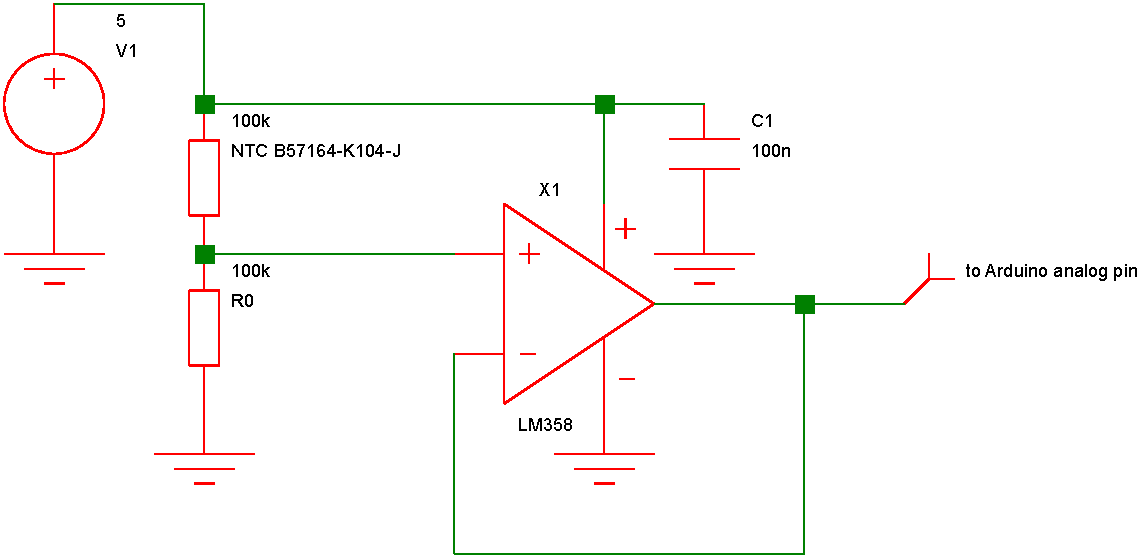
\includegraphics[width=14cm]{ntc_opamp_schematic}
\caption{Circuit for reading the NTC resistance with Op-amp.}\label{fig:tempcircuit}
\end{center}
\end{figure}

Figure \ref{fig:tempcircuit} shows the simplest possible circuit you can use for this purpose. The high input impedance of the op-amp ensures that there is basically no load on the voltage divider and we can use the simple formula which is only valid without load. There is then also virtually no current flowing through the NTC resistor which would heat it up.

%END


\subsection{Building a Heating System}\label{sec:heat}
Since it is boring to measure a constant temperature, we build a simple heat load of 0.2-0.25 W with a couple of resistors.
\begin{itemize}
	\item calculate the resistors needed to have the correct power dissipation.
	\item bring the heating resistor and the temperature sensor close together to have as good thermal contact as possible.
	\item create a plot of the temperature vs. time (starting from room temperature) and measure the time constant of the temperature rise and estimate the equilibrium temperature.
\end{itemize}

\subsection{Building a Cooling System}\label{sec:cool}
Many electrical components will produce heat under load and may break at critical temperatures. That is why many of complex systems like computers require cooling. You will now build a system that controls a fan and can regulate it's rotation speed.
\begin{itemize}
	\item connect the fan to the breadboard, for the 4 pin header, the following conventions are used:
	\begin{itemize}
	    \item black: ground
	    \item yellow: 5V
	    \item green: tacho read-out (will be used later)
	    \item blue: PWM control
	\end{itemize}
	\item keep in mind that only a few of the digital pins (marked by "{\raise.17ex\hbox{$\scriptstyle\sim$}}" on the board) are able to use PWM, e.g. use digital pin 11
\end{itemize}
Now we can finally build the full two-point controller.
\begin{itemize}
    \item define a low and high threshold, e.g. use the potentiometer for the high threshold and set the lower threshold a few degrees lower than the high one.
	\item set the duty cycle of the fan to 100\% when above the high threshold
	\item set the duty cycle of the fan to 0\% when below the low threshold
	\item setting the PWM duty-cycle can be done using the \code{analogWrite()} function
	\item if thresholds are set reasonably, you will see an oscillatory behavior. \textbf{Create a plot of temperature vs. time which shows multiple periods.}
\end{itemize}
Experiment with different set-points, what is the advantage of having two setpoints instead of a single threshold above we turn cooling on? What are the draw-backs of the two-point controller?

\subsection{Read Out the Fan Speed}
We now wan to use the built-in Hall Effect Sensor (HES) of the fan to measure its rotation speed. In every rotation this sensor will produce two pulses we can count and then convert to revolutions per minute (\textbf{RPM}). The maximum (for 100\% duty cycle) according to the datasheet is 1900 RPM, with a tolerance of 10\%, the minimum is around 230 RPM.

\begin{itemize}
	\item calculate a rough estimate for the minimum frequency needed for reading the voltage on the tacho pin and be able to count the pulses? (Use Nyquist theorem) In practice, a much higher frequency should be used than the limit calculated above
	\item check the Arduino reference of \code{analogRead()} for the maximum frequency. Since we also have to do other work in the \code{loop()} function, the frequency should be also much less than the maximum. Make a reasonable choice.
    \item what is the expected uncertainty on the minimum and maximum RPM if we count pulses for 1 second?
	\item connect the tacho (green wire) of the fan to an analog pin of the Arduino, using a 10k pull-up resistor to 5V. (optional: figure out how to use internal pull-up resistor of the Arduino instead of a discrete component)
	\item what is the role of the pull-up resistor?
	\item count the pulses of the HES and convert the result to RPM. Is it within the range expected by the datasheet numbers?
	\item write the \ac{RPM} value to the serial output
\end{itemize}

\subsection{Final measurements}
Now that our device has all basic functionalities, we can perform two additional measurements with it. For both of them disable the thresholds for the two-point controller added in the previous measurement and now vary the duty-cycle between 0 and 100\% with at least 10 steps in between.
\begin{itemize}
	\item plot the fan RPM vs. the duty cycle. Which is the minimum duty cycle above which the fan starts to spin, and at which RPM? What is the maximum RPM for full duty-cycle?
	\item plot the equilibrium temperature vs. the duty cycle and the equilibrium temperature vs. the fan RPM. Make sure you measure long enough for each data point and give a reasonable estimate for the uncertainty that you obtain on the equilibrium value.
\end{itemize}

Scanning the points for the different duty cycles should be done without flashing the device in between. Instead, the measurement programme (e.g. number of steps, seconds per step etc.) should be completely automated and either programmed into the Arduino or, alternatively, controlled by a Python program running on the computer which changes the parameters via the serial interface (see "Bi-directional communication with the computer" section below).

\textbf{After you are done with above measurement, pick one of the "Advanced" topics below or come up with your own idea. It can be a new measurement, involve new hardware, or be an improved analysis of the data measured already.}

\subsection{Building a PID Controller (Advanced)}
We have seen that with the two-point controller above, we could not exactly stabilize to a constant temperature and were suffering from under- and overshoot. Using a \ac{PID} controller can overcome both issues.
\begin{itemize}
	\item implement a \ac{PID} controller
	\item regulate cooling by the PWM duty-cycle of your fan
	\item tune your three parameters to have reasonably stable operation. (Perfect tuning is very complicated and does not have to done here.)
	\item create some plots with temperature vs. time, starting from different initial temperatures, which show converging temperature.
\end{itemize}

The output of the PID controller consists of three different terms, each having a tuneable coefficient.
\begin{itemize}
	\item proportional: proportional to the error, which is \code{error = temperature - setpoint}
	\item integral: proportional to the sum of all errors of previous steps
	\item derivative: proportional to the difference in error compared to last step
\end{itemize}

In practice, there are few more things to consider
\begin{itemize}
    \item using a timer, perform the PID calculations between every 100 ms and every second. You should not use longer values to be fast enough in response and not too much shorter values to be not susceptible to noise.
    \item use a discrete digital low-pass filter on your measured temperature if it is noisy.
    \item convert your PID response to a duty\_cycle between 0 and 255 to be used in \code{\meth{analogWrite}(\var{PIN\_FAN\_PWM}, duty\_cycle);}
\end{itemize}

A low-pass filter can be used to filter out high frequency fluctuations (noise) on the measured temperature. It can be implemented in it's simplest form with

\noindent\begin{minipage}{\textwidth}
\begin{lstlisting}[language=Arduino]
temperature = (1-LOWPASS_ALPHA) * temperature + LOWPASS_ALPHA * (temperature_current - temperature);
\end{lstlisting}
\end{minipage}

where \code{temperature\_current} is the actual reading from the sensor and \code{temperature} (which has to be properly initialized once to be the sensor reading!) the output of the filter. \code{\var{LOWPASS\_ALPHA}} controls the cut-off frequency of the lowpass filter and obviously depends on how often per seconds we measure. Set it to a reasonable value which suppresses the noise and is still fast enough for the timescale of temperature changes we expect (roughly few degrees per second). It can also be computed analytically:

\begin{equation}
\alpha = \frac{\Delta t}{\tau + \Delta t}
\end{equation}

where $\tau$ is the characteristic time constant of the low-pass filter (corresponds to RC time of a RC filter). Setting $\alpha = 0$ makes it infinitely fast, so as consequence disables the filter, where $\alpha = 1$ would make it infinitely slow, so the output would stay constant.

\subsection{Fit heating/cooling(Advanced)}
Take the two-point controller and set the two setpoints far from each other, but still in achievable range. For heating and cooling process, find a suitable function to describe the data and perform a fit of the model to data. List the fit parameters (with uncertainties!) and repeat this for several cycles. Are the uncertainties obtained by repeating the experiment consistent with the uncertainties from the fit? If not discuss why.

\subsection{Bi-directional communication with the computer (Advanced)}
Until now we only read values from the device, but we can also write commands from the computer to the Arduino using the serial interface.
\begin{itemize}
	\item instead of using the potentiometer to set the threshold, implement a way to set the threshold via serial commands
	\item one can use the SCPI protocol as a reference, e.g. set the threshold to 32 degrees with the command "SET:THR 32"
	\item which other commands are necessary to run the measurements from above section without hardcoding the measurement programme (e.g. number of steps, seconds per step etc.)?
	\item write a Python script to perform the measurements from above section via sending SCPI style commands to the Arduino
\end{itemize}


\subsection{Use of other components (Advanced)}
There is also a bunch of other components available which can be used to extend your Arduino project. Among them:
\begin{itemize}
	\item ultra-sonic distance sensor
	\item electric current sensor
	\item infrared leds and sensor
	\item electro magnet
	\item Piezzo vibration sensor
	\item 96x96 pixels OLED display
	\item Servo motor
	\item ...
\end{itemize}

Ask the assistants for more information if you are interested in using them. For example you could use the distance sensor and servo motor to keep an object at a fixed position relative to another moving one.


\subsection{I2C protocoll debugging (Advanced)}
Many of the Grove components communicate via I2C bus protocol. Using a digital oscilloscope, it is possible to look at the I2C signal and manually decode it on the scope. Use the Grove RBG LCD display, initialize it and periodically write text to the display and set the color. Spy on the commuication, find out the the device IDs of the 2 devices connected to the bus. What do they correspond to? Compare with the library of the Grove display. Record a short communication of a few bytes and decode it.















